\chapter{Run-length compressed suffix array}\label{chapter:rlcsa}

In the terminology of Chapter~\ref{chapter:csa}, the \emph{run-length compressed suffix array (RLCSA)} is a compressed self-index of the CSA family using data-aware run-length encoded bit vectors. As a theoretical structure, RLCSA has been described and analyzed in Paper~I. Many of the implementation choices have been described in Paper~II.

RLCSA has been designed for indexing highly repetitive sequences or collections of sequences. A sequence can be considered highly repetitive, if the number of equal letter runs in the Burrows-Wheeler transform is much less than the length of the sequence. Run-length encoding achieves good compression in such cases, if the bit vectors and other structures are data-aware, with no significant dependencies on the length of the sequence in their size bounds. Other design principles include simplicity and practical efficiency, even when a more complicated design might provide better theoretical time or space bounds.

In some sense, RLCSA is a a data-aware variant of Sad-CSA. Paper~I also describes data-aware versions of RLFM and SSA, designed and implemented by Niko Välimäki. The \emph{improved run-length FM-index (RLFM+)} uses the bit vector of Gupta \etal{Gupta2007} to encode the lengths of equal letter runs, but is otherwise identical to the original RLFM. The \emph{run-length encoded wavelet tree (RLWT)} is based on a balanced wavelet tree, using two gap encoded bit vectors of Gupta \etal{Gupta2007} per binary sequence to achieve run-length encoding. While all three indexes have similar space bounds, RLWT is slightly smaller than RLCSA in practice, while RLFM+ is clearly larger. On the other hand, RLCSA is the fastest of the three indexes, followed by RLFM+ and RLWT.
\newpage

\section{Analysis}\label{sect:rlcsa analysis}

RLCSA uses data-aware run-length encoded and gap encoded bit vectors. Technical details of these bit vectors are described in Section~\ref{sect:rlcsa implementation}. For the theoretical analysis, it is enough to note that both bit vectors support \rank\ and \select\ in $O(\log n + b)$ time, where $b$ is the size of small blocks in bits. On a binary sequence $B$ of length $n$, with $n_{1}$ \onebit{}s in $R_{1}$ runs, the size bounds are
$$
\left( \gap(B) + O\left( n_{1} \log \log \frac{n}{n_{1}} \right) \right)
\left( 1 + \frac{O(\log n)}{b} \right)
$$
bits for the gap encoded variant and
$$
\left( \run(B) + O\left( R_{1} \log \log \frac{n}{R_{1}} \right) \right)
\left( 1 + \frac{O(\log n)}{b} \right)
$$
bits for the run-length encoded variant.

Assume that there are $R$ equal letter runs in the Burrows-Wheeler transform. Then the total number of runs of \onebit{}s in bit vectors $B_{c}$ is also $R$. As the total number of \onebit{}s is $n$ and the total number of \zerobit{}s is $(\sigma - 1) n$, we get a size bound of
$$
R
\left( \log \frac{\sigma n}{R} + \log \frac{n}{R} + O\left( \log\log \frac{\sigma n}{R} \right) \right)
\left( 1 + \frac{O(\log n)}{b} \right)
$$
bits for BWT by using the bound $\gap \le n_{1} \log (n / n_{1}) + n_{1}$. This size bound has an extra $R \log (n/R)$ term, when compared to direct run-length encoding of the BWT (see Section~\ref{sect:compression}), as we are encoding the runs of each character separately.

We use the sampling scheme described in Section~\ref{sect:full functionality} to support \locate\ and \extract. A gap encoded bit vector is used as $B_{s}$ to mark the sampled positions. With sample rate $d$, the total size of the samples is $O((n/d) \log (n/d))$ bits. Gap encoded bit vectors are also used for encoding array $C$ and marking sequence boundaries. Together with the overhead from alphabet size and the number of sequences, these bit vectors take $O((r + \sigma) \log n)$ bits, where $r$ is the number of sequences in the collection. From Theorem~\ref{theorem:csa}, we get the following theorem.

\begin{theorem}\label{theorem:rlcsa}
Assume we have a collection of $r$ texts with total length $N$. The run-length compressed suffix array for the collection takes
\begin{multline*}
R
\left( \log \frac{\sigma N}{R} + \log \frac{N}{R} + O\left( \log\log \frac{\sigma N}{R} \right) \right)
\left( 1 + \frac{O(\log N)}{b} \right) \\
+ O\left( \frac{N}{d} \log \frac{N}{d} + (r + \sigma) \log N \right)
\end{multline*}
bits of space, where $b$ is the block size in bits, $R$ is the number of equal letter runs in the Burrows-Wheeler transform of the collection, and $d$ is the suffix array sample rate. The index supports \find$(P)$ in $O(\abs{P} \cdot (\log N + b))$ time, \locate\ in $O(d \cdot (\log N + b))$ time, and \extract$(i,j)$ in $O((d + j - i) (\log N + b))$ time.
\end{theorem}

In practice, block size $b$ is chosen to be $\Theta(\log N)$ bits, so that the factor $1 + O(\log N) / b$ in the size bound becomes $1 + \varepsilon$, for some constant $0 < \varepsilon < 1$. This also simplifies the factor $\log N + b$ in the time bounds to $O(\log N)$.


\section{Runs in BWT}\label{sect:runs}

In Section~\ref{sect:full-text indexes}, we defined that each sequence of a collection has a distinct end marker, making the set of suffixes of the collection well-ordered. A drawback of this definition is that it increases the alphabet size significantly for large collections. In the following analysis, as well as in practice, we avoid the drawback replacing all end markers with a single symbol $\$$ after sorting. By doing this, we lose the ability to compute $\Psi$ for suffix array positions corresponding to the end markers, as well as the ability to compute $LF$ for positions corresponding to the first characters of a sequence.

\paragraph{Entropy-based estimates.}

As noted in Section~\ref{sect:compression}, the number of equal letter runs in the BWT of a text of length $n$ is $R(T) \le nH_{k}(T') + w_{k}(T')$, where $T'$ is the reverse of text $T$ and $w_{k}(T')$ is the number of \orderk{k} contexts occurring in the reverse text. This bound holds simultaneously for all $k \ge 0$.

If we assume that the text has been generated by an \orderk{0} source, we can use the character frequencies to approximate the expected number of runs. The character at position $i$ in the Burrows-Wheeler transform is a run head, if $i = 1$ or if the suffixes with lexicographic ranks $i-1$ and $i$ are preceded by different characters. Assuming that the character distribution is $\mathbf{p} = [n_{1}/n, \cdots, n_{\sigma}/n]$, the probability that the preceding characters differ is $1 - \mathbf{p} \cdot \mathbf{p}$. Hence we can estimate that for an \orderk{0} source, $R \approx n(1 - \mathbf{p} \cdot \mathbf{p})$. Similar estimates can be made for higher order sources as well.

\paragraph{Highly repetitive collections.}

For $k = \lceil \log_{\sigma} n \rceil$, the number of possible \orderk{k} contexts is $\sigma^{k} \ge n$. If a significant fraction of these contexts occur in the text, then the model will probably take more space than a statistical encoding of the text based on that model. Hence it is not reasonable to use an \orderk{k'} model, for $k' > k$, to describe the text, unless only a small fraction of the possible contexts occur in the text, making it highly repetitive. On the other hand, if the number of runs is significantly less than predicted by an \orderk{k} model, lexicographically adjacent suffixes will likely be preceded by the same character, making the text highly repetitive.

\begin{definition}
A collection of texts with total length $N$ is \emph{highly repetitive}, if the number of equal letter runs in the Burrows-Wheeler transform of the collection is significantly less than predicted by an \orderk{k} model, for $k = \lceil \log_{\sigma} N \rceil$.
\end{definition}

In the following, we estimate the number of equal letter runs in the Burrows-Wheeler transform of a highly repetitive collection, created by applying $s$ random edit operations on a collection of $r$ identical random texts of length $n$.

\paragraph{Combinatorial properties.}

\begin{lemma}\label{lemma:runs for copies}
Let $\mathcal{C} = \set{T_{1}, \dotsc, T_{r}}$ be a collection of $r$ copies of text $T$. Then $R(\mathcal{C}) = R(T)$.
\end{lemma}

\begin{proof}
For all positions $j$, the suffixes $T_{i}[j,n]$ and $T_{i'}[j,n]$ are identical for any texts $T_{i}$ and $T_{i'}$, and the lexicographic order among them is determined by sequence numbers. Hence $\mrank(\mathcal{C}, T_{i}[j,n]) = r \cdot (\mrank(T, T[j,n]) - 1) + i$. As the suffixes $T_{i}[j-1,n]$ are also identical for all texts $T_{i}$, we have
$$
\BWT_{\mathcal{C}}[\mrank(\mathcal{C}, T_{1}[j,n]), \mrank(\mathcal{C}, T_{r}[j,n])] =
\BWT_{T}[\mrank(T, T[j,n])]^{r}.
$$
Hence the number of equal letter runs does not depend on the number of copies of text $T$.
\end{proof}

\begin{definition}
Let $\mathcal{C} = \set{T_{1}, \dotsc, T_{r}}$ be a collection of texts, all derived by substitutions, insertions, and deletions from some base text $T$, and let $\mathcal{A}$ be a multiple alignment representing those edit operations. The \emph{significant prefix} $S_{i,j}$ of suffix $T_{i}[j,\abs{T_{i}}]$ is the shortest prefix of $T_{i}[j,\abs{T_{i}}]$ that differentiates it from all other suffixes, except possibly from those with first characters aligned with character $T_{i}[j]$.
\end{definition}

The intuition behind the definition is that significant prefixes can be used to sort non-aligned suffixes into lexicographic order. Aligned suffixes are assumed to be equivalent in respect to the number of runs, unless there has been an edit operation nearby.

\begin{lemma}\label{lemma:one mutation}
Let $\mathcal{C} = \set{T_{1}, \dotsc, T_{r}}$ be a collection of $r$ copies of text $T$, and let $\mathcal{C'}$ be the same collection after substituting one character of one text with another character. Then $R(\mathcal{C'}) \le R(T) + O(k)$, where $k$ is the number of suffixes of collection $\mathcal{C'}$ whose significant prefixes cover the substitution.
\end{lemma}

\begin{proof}
Assume that the substituted character was $T_{i}[j]$. We get the new Burrows-Wheeler transform $\BWT_{\mathcal{C'}}$ by removing the characters corresponding to suffixes $T_{i}[1,n], \dotsc, T_{i}[j+1,n]$ from $\BWT_{\mathcal{C}}$ and inserting them into their new positions, as the rest of the suffixes remain the same.

As $k$ significant prefixes cover the substituted character, suffixes $T_{i}[1,n]$ to $T_{i}[j-k,n]$ are not affected by the substitution. The lexicographic order between them and the remaining non-aligned suffixes does not change. The lexicographic order between a removed suffix and aligned suffixes can change, but as the preceding character does not change, this means just inserting the same character back into a different part of the same run. Hence we only need to consider suffixes $T_{i}[j-k+1,n]$ to $T_{i}[j+1,n]$.

For suffixes $T_{i}[j-k+1,n]$ to $T_{i}[j,n]$, we are inserting the same character into a new position in the BWT. This can break an existing run into two parts, and the inserted character can create another run on its own. Hence these suffixes can create at most $2k$ new runs. Finally we insert the substituted character to the original position of suffix $T_{i}[j+1,n]$. This can also break an existing run and create a new run, so the total number of new runs is at most $2k+2$. The result follows by noting that according to Lemma~\ref{lemma:runs for copies}, $R(\mathcal{C}) = R(T)$.
\end{proof}

The lemma immediately generalizes to multiple substitutions.

\begin{corollary}\label{corollary:many mutations}
Let $\mathcal{C} = \set{T_{1}, \dotsc, T_{r}}$ be a collection of $r$ copies of text $T$, and let $\mathcal{C'}$ be the same collection after substituting a total of $s$ characters with other characters. Then $R(\mathcal{C'}) \le R(T) + O(k)$, where $k$ is the number of suffixes of collection $\mathcal{C'}$ whose significant prefixes cover at least one substitution.
\end{corollary}

\begin{proof}
The proof follows that of Lemma~\ref{lemma:one mutation}. For each substitution $T_{i}[j]$, we remove the characters corresponding to suffixes whose significant prefixes contain the substitution, and insert them into their new positions.
\end{proof}

\paragraph{Expected case properties.}

In the following, we assume that all random choices are independent and identically distributed.

\begin{lemma}\label{lemma:longest repeat}
Let $T$ be a random text. The expected length of the longest repeated substring is $O(\log_{\sigma} n)$.
\end{lemma}

\begin{proof}
Let $X_{i,j}^{k}$, where $i < j \le n-k+1$, be a variable indicating whether substrings $T[i,i+k-1]$ and $T[j,j+k-1]$ are identical. If $i+k \le j$, the expected value of $X_{i,j}^{k}$ is $\sigma^{-k}$.

Consider now the case $j < i+k$, where the substrings overlap at $k - (j-i)$ positions. To get identical substrings, we can choose $T[i,j-1]$ arbitrarily, but character $T[l]$ must be identical to $T[l - (j-i)]$ for all $j \le l < j+k$. Hence the expected value of $X_{i,j}^{k}$ is also $\sigma^{-k}$ in this case.

The expected number of repeats of length $k$ is then
$$
E\left[ \sum_{1 \le i < j \le n-k+1} X_{i,j}^{k} \right] \le \frac{n^{2}}{2 \sigma^{k}}.
$$
By Markov's inequality, the probability of having at least one repeat of length $2 \log_{\sigma} n + k'$ is at most $1/(2 \sigma^{k'})$. As the probability decreases exponentially by $k'$, the expected length of the longest repeat is $O(\log_{\sigma} n)$.
\end{proof}

We are now ready to prove the main result.

\begin{theorem}\label{theorem:expected case runs}
Let $\mathcal{C} = \set{T_{1}, \dotsc, T_{r}}$ be a collection of $r$ copies of random text $T[1,n]$ over alphabet of size $\sigma$, and let $\mathcal{C'}$ be the same collection after randomly substituting a total of $s$ characters with other characters. Then the expected number of runs in the Burrows-Wheeler transform of collection $\mathcal{C'}$ is at most $R(T) + O(s \log_{\sigma} (rn))$.
\end{theorem}

\begin{proof}
Consider texts $T_{i}$ and $T_{i'}$ of collection $\mathcal{C'}$, and some arbitrary positions $j < j'$ in them. If the substring of length $k$ starting at $T_{i}[j]$ is identical to the one starting at $T_{i'}[j']$, then the corresponding suffixes must have significant prefixes of length at least $k+1$. By following the proof of Lemma~\ref{lemma:longest repeat}, we find that the expected length of the longest such repeat is $O(\log_{\sigma} (rn))$, so significant prefixes of length $O(\log_{\sigma} (rn))$ are enough in the expected case. The result follows from Corollary~\ref{corollary:many mutations}.
\end{proof}

\paragraph{Extensions.}

While above results consider only substitutions, they are easy to extend to handle random insertions and arbitrary deletions. If an insertion happens after character $T_{i}[j]$, and suffix $T_{i}[j-k+1,n]$ is the longest one whose significant prefix covers at least one of the inserted characters, then we have to remove suffixes $T_{i}[j-k+1,n]$ to $T_{i}[j+1,n]$, and insert them to their new positions, along with the new suffixes. Similarly, if we delete substring $T_{i}[j,j']$, we remove suffixes $T_{i}[j-k+1,n]$ to $T_{i}[j'+1,n]$, and insert the ones that were not deleted to their new positions.

Large insertions consisting of a substring already in the collection are also easy to handle. A \emph{recombination}, replacing texts $T_{1} = T_{1,a} T_{1,b}$ and $T_{2} = T_{2,a} T_{2,b}$ with texts $T_{1,a} T_{2,b}$ and $T_{2,a} T_{1,b}$, is essentially two edit operations. Extending a text by a LZ77 phrase consisting of a substring already occurring in the collection, followed by a single character, is also worth two edit operations. In general, we can estimate the effect of a complex edit operation on the number of runs by counting the \emph{points of discontinuity} the operation introduces into the collection, and treating each of them as a simple edit operation.


\section{Implementation}\label{sect:rlcsa implementation}

The implementation of RLCSA has been written in C++. All queries have been implemented as \texttt{const} functions that do not alter the state of the index, allowing multiple threads to to use the index in parallel. Index construction (see Chapter~\ref{chapter:construction}) has also been parallelized by using \emph{OpenMP} and either \emph{MCSTL}\footnote{\url{http://algo2.iti.kit.edu/singler/mcstl/}} or the version of MCSTL integrated into GCC, the \emph{libstdc++ parallel mode}.

Both gap encoded and run-length encoded bit vectors support a number of derived queries in addition to the plain \rank\ and \select. For example, $\operatorname{valueAfter}(i)$ returns $(i', \mrank_{1}(B, i'))$ for the smallest $i' \ge i$ such that $B[i'] = 1$. Iterator version of \select\ allows calling \select\ for successive \onebit{}s faster than by using the plain query. Another variant $\operatorname{selectRun}(i)$ returns the length of the run of \onebit{}s starting from the one of rank $i$, in addition to answering \select.

Small blocks consist of $b$ bits of compressed data. In gap encoded bit vectors, the compressed data consists of $\delta$\nobreakdash-encoded distances between successive \onebit{}s. If a code does not fit into the current block, it is stored in the next block, and the rest of the block remains empty. In run-length encoded bit vectors, each run is encoded as the distance from the previous run, followed by the number of \onebit{}s in the run. Both of the integers are encoded using \deltacode{}s, as they are expected to be fairly large in highly repetitive sequences (see Sections~\ref{sect:bit vectors} and \ref{sect:runs}). The entire encoding of a run must fit into the block, or else it is stored in the next block. However, a maximal run of \onebit{}s can be split into two shorter runs, so that the first of these runs can be stored in the last remaining bits of a block.

For each small block, the first \onebit{} $B[i]$ not included in the previous blocks is sampled and stored as a pair $(i, \mrank_{1}(B, i))$ taking $2 \lceil \log (n+1) \rceil$ bits, where $n$ is the length of the binary sequence. This sample is not included in the corresponding block. Separate large blocks are used for \rank\ and \select. In both cases, the parameter space ($[1,n]$ for \rank\ and $[1,n_{1}]$ for \select) is divided into $n_{b} / 5$ blocks of equal size, where $n_{b}$ is the number of small blocks. For each large block containing the range $[a,a']$ of parameter space, we store a pointer to the small block that is used to answer $\mrank_{1}(B,a)$ or $\mselect_{1}(B,a)$. Each of these pointers takes $\lceil \log (n_{b}+1) \rceil$ bits.

To answer $\mrank_{1}(B,i)$ or $\mselect_{1}(B,i')$, we start by dividing the parameter by the length of a large block. This gives us $j$, the number of the large block that contains the answer to the query. Pointers for large blocks $j$ and $j+1$ give us the range of small blocks that contains the answer, and the correct block is determined by binary searching the sampled \onebit{}s corresponding to these small blocks. Finally, the small block is decompressed to determine the answer. Finding the correct small block takes $O(\log n)$ time, and decompressing the block takes $O(b)$ time. The number of random memory accesses is $3$, unless the large block contains many small blocks.

The implementation uses linear search instead of binary search to find the small block. This does not guarantee performance in the worst case, but is faster in practice. If the binary sequence is very skewed, some large blocks can contain many small blocks, reducing query performance for those blocks. While this behavior has been seen in practice, the effect seems to be limited on real data \cite{Ferragina2011}.

RLCSA uses the standard sampling mechanism (see Section~\ref{sect:full functionality}) to support \locate\ and \extract. In addition to locating a single position at a time, the implementation also contains a variant of \locate\ that locates all positions in a suffix array range simultaneously. This version is often several times faster than the standard one, taking advantage of both memory locality and the run-length encoding in the bit vectors. In addition to selecting samples at regular intervals, it is also possible to select the samples optimally or greedily according to a known query distribution \cite{Ferragina2011}.

Default small block sizes are $32$ bytes for the run-length encoded bit vectors and $16$ bytes for the gap encoded ones. Suffix array sample rate $d$ defaults to $128$, with samples taking less than $n$ bits for a sequence of length $n$. Instead of using a bit vector, array $C$ has been implemented with an ad hoc mechanism that is somewhat similar to the high level structure in bit vectors, but faster in practice. Alphabet has been fixed to $0, \dotsc, 255$, where $0$ plays the role of end marker $\$$ in some construction options, while being a regular character in other alternatives.

Support for multiple sequences is based on having different lexicographic values for the end markers of different sequences, as described in Section~\ref{sect:full-text indexes}. The sequences are implicitly concatenated to form a single sequence, and a bit vector is used to map positions in this sequence to actual sequences. Some padding is added to between the sequences, so that a new sequence always starts at a position that is a multiple of sample rate $d$. This way, the regular sampling mechanism always samples the first position of every sequence. The end marker of each sequence is implicitly sampled, as its lexicographic rank corresponds to the sequence number.
\newpage


\section{Experiments}\label{sect:rlcsa experiments}

In this section, we compare the size and query performance of RLCSA to \sadcsa\ (see Section~\ref{sect:bit vectors}), the most similar earlier self-index. We chose two highly repetitive data sets: the genomes of 36 strains of \emph{Saccharomyces paradoxus} (para) from Paper~I, taking a total of 409 megabytes, and a 400-megabyte prefix of the Finnish language Wikipedia archive with full version history from Paper~II. The experiments were performed on a system with two quad-core 2.53 GHz Intel Xeon E5540 processors running Ubuntu 10.04 with Linux kernel 2.6.32. Only one core was used in the experiments. The programs were compiled with g++ version 4.4.3. For a more thorough experimental comparison, see Paper~I.

We measured \find\ and \locate\ (including \find) performance of the indexes with $50000$ randomly selected patterns of length $20$. The indexes used default parameter values and suffix array sample rates $d = 32, 64, 128, 256$. In RLCSA, we used both the standard \locate\ mechanism (RLCSA) and the one optimized for locating ranges of suffix array values (RLCSA\nobreakdash-OPT).

Index sizes and \find\ results can be seen in Table~\ref{table:rlcsa}. Of the two data sets, fiwiki turned out to be much more repetitive. RLCSA was able to compress it to just $1.6\%$ of the original size, while the non-data-aware \sadcsa\ required more than $13\%$ of the original size. On para, the differences were smaller, with RLCSA taking $10\%$ and \sadcsa\ $17\%$ of the original size. The \find\ performance of RLCSA was much better than that of \sadcsa, as the compressed representation of $\Psi$ in \sadcsa\ does not support \rank\ directly, but uses binary search on \select\ instead.

\begin{table}
\centering
\renewcommand{\tabcolsep}{.1cm}
\begin{tabular}{lccccccc}
\hline\noalign{\smallskip}
 & & & \multicolumn{2}{c}{\textbf{RLCSA}} & & \multicolumn{2}{c}{\textbf{\sadcsa}} \\
\textbf{Data set} & \textbf{Size} & & \textbf{Size} & \textbf{Find} & & \textbf{Size} & \textbf{Find} \\ 
\noalign{\smallskip}
\hline
\noalign{\smallskip}
para   & 409 MB & & 41.34 MB & 1.12 MB/s & & 69.92 MB & 0.34 MB/s \\
fiwiki & 400 MB & &  5.63 MB & 1.36 MB/s & & 53.05 MB & 0.38 MB/s \\
\noalign{\smallskip}
\hline
\end{tabular}

\caption{RLCSA and \sadcsa\ for two highly repetitive collections. Index size without suffix array samples and \find\ performance on $50000$ patterns of length $20$.}\label{table:rlcsa}
\end{table}

The results for \locate\ can be seen in Figure~\ref{fig:rlcsa}. RLCSA with optimized \locate\ is faster than \sadcsa\ with the same sample rate, and also much smaller. With regular \locate, RLCSA loses to \sadcsa, especially on the more repetitive fiwiki data set. As both indexes are much faster on fiwiki than on para, the implementation of \sadcsa\ seems to have some optimizations for locating suffix array ranges simultaneously as well.

\begin{figure}
\centerline{
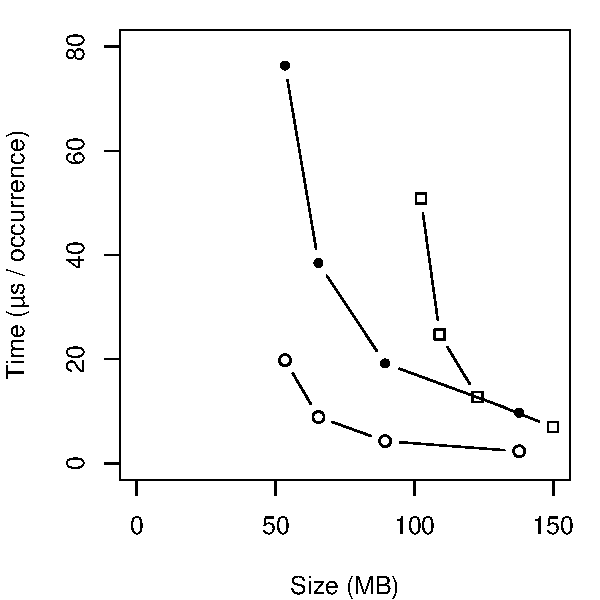
\includegraphics[width=.45\textwidth]{experiments/rlcsa/locate_para.pdf}
\hspace{5pt}
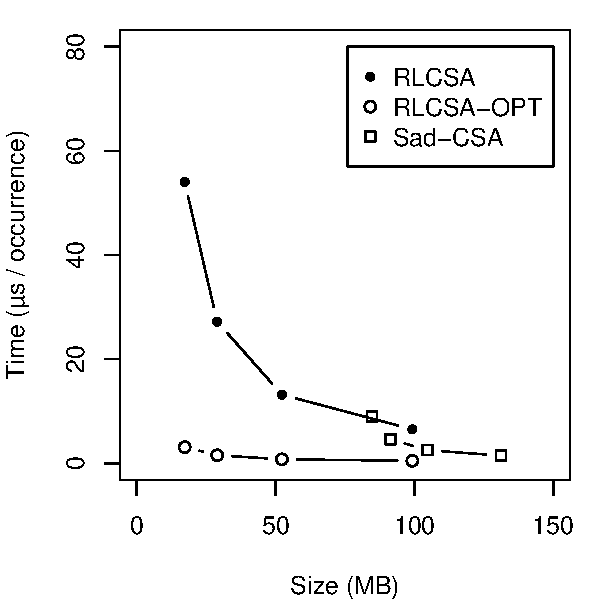
\includegraphics[width=.45\textwidth]{experiments/rlcsa/locate_fiwiki.pdf}
}

\caption{\emph{Locate} performance of RLCSA and \sadcsa\ on para (left) and fiwiki (right). Index sizes and average \locate\ times with sample rates $d = 32, 64, 128, 256$ on $50000$ patterns of length $20$.}\label{fig:rlcsa}
\end{figure}

The optimized \locate\ is $13$--$18$ times faster than the standard one on fiwiki, and about $4$ times faster on para. This shows that even though RLCSA is unable to compress the samples, unlike some other proposals \cite{Maekinen2010,Huang2010}, it can compensate this by using a small number of samples more efficiently, when the collection is highly repetitive.

In general, the optimizations depend on both the number and the length of the repetitions. Assume that we want to locate a pattern that occurs at the beginning of a repeated substring of length $l$, with $k$ copies in the collection. Then $k$ is an upper bound for the speedup from the optimizations, and the actual speedup depends on whether the significant prefixes of the sampled suffixes used in the \locate\ are within the repeated substring. If this is the case, then the suffixes remain lexicographically adjacent until the samples have been found. Otherwise the suffixes diverge at some point, limiting the speedup from locating all occurrences simultaneously.

It should be noted that \sadcsa\ has been optimized for \locate. The small blocks in the encoding of $\Psi$ contain a fixed number of values (\onebit{}s) each, and hence the correct block can be derived directly from the parameter value, avoiding one level of indirection. The sampling mechanism is also non-standard, storing one out of $d$ suffix array values instead of one out of $d$ text positions. This does not guarantee worst-case time bounds, but makes it much faster to determine whether the current suffix array value has been sampled.
\newpage


\section{Later indexes}

RLCSA was the first compressed index that was intended for indexing highly repetitive collections. Later papers on similar topics have used it as a reference point, against which the authors compare their results.

The self-index of Huang \etal{Huang2010} is based on a multiple alignment of similar sequences. The authors start with similar analysis as in Section~\ref{sect:runs}, and explicitly encode the differences between the sequences, while building a BWT-based index for the common segments in the sequences. When the number of differences is small, the index is smaller than RLCSA. The main reason for this is that the common segments are stored just once, while RLCSA uses $O(\log r)$ extra bits per run to encode the $r$ copies. Because of the complexity of the index, \find\ is slower than in regular BWT-based indexes. On the other hand, \locate\ can be much faster, if the pattern occurs mostly in the common segments.

The work of Claude \etal{Claude2009,Claude2010} develops self-indexes based on \emph{straight-line programs (SLP)} in general, and \emph{Re\nobreakdash-Pair} \cite{Larsson1999} in particular. Similar to \lzindex{}es, these indexes offer fast \locate, but do not support \find. A straight-line program is essentially a \emph{context-free grammar} in the \emph{Chomsky normal form} for a language containing a single sequence. In the grammar, each variable $X$ produces either two new variables $YZ$ or a character $c \in \Sigma$. One variant compresses the text with Re\nobreakdash-Pair, allowing fast random access to it, and uses a \emph{$q$\nobreakdash-gram index}, where the occurrence lists are differentially encoded and compressed with LZ77. Another variant uses the Re\nobreakdash-Pair encoding of the text directly as a self-index. Both variants offer better compression than RLCSA, if the text is very highly repetitive \cite{Claude2010}.

As already conjectured in the original paper describing RLCSA, a self-index based on LZ77 parsing offers better compression for highly repetitive sequences than RLCSA. The LZ77\nobreakdash-index of Kreft and Navarro \cite{Kreft2011} proves this conjecture. Like the other \lzindex{}es, the index is much larger than plain LZ77-compressed text. In practice, the LZ77\nobreakdash-index is smaller and offers faster \locate\ than RLCSA and SLP-based indexes on highly repetitive texts. The reason for better compression than SLP-based indexes is that while both approaches replace a repetition with a reference, SLPs have more overhead in encoding the original copy.

There have also been recent papers on compressing highly repetitive collections of sequences, while supporting the decompression of individual sequences or arbitrary substrings efficiently \cite{Kuruppu2010,Ferragina2010a,Kreft2010}. In these tasks, RLCSA is at disadvantage, as LZ77 compresses highly repetitive texts better than BWT, and the bit vector-based encoding of BWT also adds some overhead, when compared to direct compression. 
